% Options for packages loaded elsewhere
\PassOptionsToPackage{unicode}{hyperref}
\PassOptionsToPackage{hyphens}{url}
\PassOptionsToPackage{dvipsnames,svgnames,x11names}{xcolor}
%
\documentclass[
  letterpaper,
  DIV=11,
  numbers=noendperiod]{scrartcl}

\usepackage{amsmath,amssymb}
\usepackage{lmodern}
\usepackage{iftex}
\ifPDFTeX
  \usepackage[T1]{fontenc}
  \usepackage[utf8]{inputenc}
  \usepackage{textcomp} % provide euro and other symbols
\else % if luatex or xetex
  \usepackage{unicode-math}
  \defaultfontfeatures{Scale=MatchLowercase}
  \defaultfontfeatures[\rmfamily]{Ligatures=TeX,Scale=1}
\fi
% Use upquote if available, for straight quotes in verbatim environments
\IfFileExists{upquote.sty}{\usepackage{upquote}}{}
\IfFileExists{microtype.sty}{% use microtype if available
  \usepackage[]{microtype}
  \UseMicrotypeSet[protrusion]{basicmath} % disable protrusion for tt fonts
}{}
\makeatletter
\@ifundefined{KOMAClassName}{% if non-KOMA class
  \IfFileExists{parskip.sty}{%
    \usepackage{parskip}
  }{% else
    \setlength{\parindent}{0pt}
    \setlength{\parskip}{6pt plus 2pt minus 1pt}}
}{% if KOMA class
  \KOMAoptions{parskip=half}}
\makeatother
\usepackage{xcolor}
\setlength{\emergencystretch}{3em} % prevent overfull lines
\setcounter{secnumdepth}{-\maxdimen} % remove section numbering
% Make \paragraph and \subparagraph free-standing
\ifx\paragraph\undefined\else
  \let\oldparagraph\paragraph
  \renewcommand{\paragraph}[1]{\oldparagraph{#1}\mbox{}}
\fi
\ifx\subparagraph\undefined\else
  \let\oldsubparagraph\subparagraph
  \renewcommand{\subparagraph}[1]{\oldsubparagraph{#1}\mbox{}}
\fi

\usepackage{color}
\usepackage{fancyvrb}
\newcommand{\VerbBar}{|}
\newcommand{\VERB}{\Verb[commandchars=\\\{\}]}
\DefineVerbatimEnvironment{Highlighting}{Verbatim}{commandchars=\\\{\}}
% Add ',fontsize=\small' for more characters per line
\usepackage{framed}
\definecolor{shadecolor}{RGB}{241,243,245}
\newenvironment{Shaded}{\begin{snugshade}}{\end{snugshade}}
\newcommand{\AlertTok}[1]{\textcolor[rgb]{0.68,0.00,0.00}{#1}}
\newcommand{\AnnotationTok}[1]{\textcolor[rgb]{0.37,0.37,0.37}{#1}}
\newcommand{\AttributeTok}[1]{\textcolor[rgb]{0.40,0.45,0.13}{#1}}
\newcommand{\BaseNTok}[1]{\textcolor[rgb]{0.68,0.00,0.00}{#1}}
\newcommand{\BuiltInTok}[1]{\textcolor[rgb]{0.00,0.23,0.31}{#1}}
\newcommand{\CharTok}[1]{\textcolor[rgb]{0.13,0.47,0.30}{#1}}
\newcommand{\CommentTok}[1]{\textcolor[rgb]{0.37,0.37,0.37}{#1}}
\newcommand{\CommentVarTok}[1]{\textcolor[rgb]{0.37,0.37,0.37}{\textit{#1}}}
\newcommand{\ConstantTok}[1]{\textcolor[rgb]{0.56,0.35,0.01}{#1}}
\newcommand{\ControlFlowTok}[1]{\textcolor[rgb]{0.00,0.23,0.31}{#1}}
\newcommand{\DataTypeTok}[1]{\textcolor[rgb]{0.68,0.00,0.00}{#1}}
\newcommand{\DecValTok}[1]{\textcolor[rgb]{0.68,0.00,0.00}{#1}}
\newcommand{\DocumentationTok}[1]{\textcolor[rgb]{0.37,0.37,0.37}{\textit{#1}}}
\newcommand{\ErrorTok}[1]{\textcolor[rgb]{0.68,0.00,0.00}{#1}}
\newcommand{\ExtensionTok}[1]{\textcolor[rgb]{0.00,0.23,0.31}{#1}}
\newcommand{\FloatTok}[1]{\textcolor[rgb]{0.68,0.00,0.00}{#1}}
\newcommand{\FunctionTok}[1]{\textcolor[rgb]{0.28,0.35,0.67}{#1}}
\newcommand{\ImportTok}[1]{\textcolor[rgb]{0.00,0.46,0.62}{#1}}
\newcommand{\InformationTok}[1]{\textcolor[rgb]{0.37,0.37,0.37}{#1}}
\newcommand{\KeywordTok}[1]{\textcolor[rgb]{0.00,0.23,0.31}{#1}}
\newcommand{\NormalTok}[1]{\textcolor[rgb]{0.00,0.23,0.31}{#1}}
\newcommand{\OperatorTok}[1]{\textcolor[rgb]{0.37,0.37,0.37}{#1}}
\newcommand{\OtherTok}[1]{\textcolor[rgb]{0.00,0.23,0.31}{#1}}
\newcommand{\PreprocessorTok}[1]{\textcolor[rgb]{0.68,0.00,0.00}{#1}}
\newcommand{\RegionMarkerTok}[1]{\textcolor[rgb]{0.00,0.23,0.31}{#1}}
\newcommand{\SpecialCharTok}[1]{\textcolor[rgb]{0.37,0.37,0.37}{#1}}
\newcommand{\SpecialStringTok}[1]{\textcolor[rgb]{0.13,0.47,0.30}{#1}}
\newcommand{\StringTok}[1]{\textcolor[rgb]{0.13,0.47,0.30}{#1}}
\newcommand{\VariableTok}[1]{\textcolor[rgb]{0.07,0.07,0.07}{#1}}
\newcommand{\VerbatimStringTok}[1]{\textcolor[rgb]{0.13,0.47,0.30}{#1}}
\newcommand{\WarningTok}[1]{\textcolor[rgb]{0.37,0.37,0.37}{\textit{#1}}}

\providecommand{\tightlist}{%
  \setlength{\itemsep}{0pt}\setlength{\parskip}{0pt}}\usepackage{longtable,booktabs,array}
\usepackage{calc} % for calculating minipage widths
% Correct order of tables after \paragraph or \subparagraph
\usepackage{etoolbox}
\makeatletter
\patchcmd\longtable{\par}{\if@noskipsec\mbox{}\fi\par}{}{}
\makeatother
% Allow footnotes in longtable head/foot
\IfFileExists{footnotehyper.sty}{\usepackage{footnotehyper}}{\usepackage{footnote}}
\makesavenoteenv{longtable}
\usepackage{graphicx}
\makeatletter
\def\maxwidth{\ifdim\Gin@nat@width>\linewidth\linewidth\else\Gin@nat@width\fi}
\def\maxheight{\ifdim\Gin@nat@height>\textheight\textheight\else\Gin@nat@height\fi}
\makeatother
% Scale images if necessary, so that they will not overflow the page
% margins by default, and it is still possible to overwrite the defaults
% using explicit options in \includegraphics[width, height, ...]{}
\setkeys{Gin}{width=\maxwidth,height=\maxheight,keepaspectratio}
% Set default figure placement to htbp
\makeatletter
\def\fps@figure{htbp}
\makeatother

\KOMAoption{captions}{tableheading}
\makeatletter
\makeatother
\makeatletter
\makeatother
\makeatletter
\@ifpackageloaded{caption}{}{\usepackage{caption}}
\AtBeginDocument{%
\ifdefined\contentsname
  \renewcommand*\contentsname{Table of contents}
\else
  \newcommand\contentsname{Table of contents}
\fi
\ifdefined\listfigurename
  \renewcommand*\listfigurename{List of Figures}
\else
  \newcommand\listfigurename{List of Figures}
\fi
\ifdefined\listtablename
  \renewcommand*\listtablename{List of Tables}
\else
  \newcommand\listtablename{List of Tables}
\fi
\ifdefined\figurename
  \renewcommand*\figurename{Figure}
\else
  \newcommand\figurename{Figure}
\fi
\ifdefined\tablename
  \renewcommand*\tablename{Table}
\else
  \newcommand\tablename{Table}
\fi
}
\@ifpackageloaded{float}{}{\usepackage{float}}
\floatstyle{ruled}
\@ifundefined{c@chapter}{\newfloat{codelisting}{h}{lop}}{\newfloat{codelisting}{h}{lop}[chapter]}
\floatname{codelisting}{Listing}
\newcommand*\listoflistings{\listof{codelisting}{List of Listings}}
\makeatother
\makeatletter
\@ifpackageloaded{caption}{}{\usepackage{caption}}
\@ifpackageloaded{subcaption}{}{\usepackage{subcaption}}
\makeatother
\makeatletter
\@ifpackageloaded{tcolorbox}{}{\usepackage[many]{tcolorbox}}
\makeatother
\makeatletter
\@ifundefined{shadecolor}{\definecolor{shadecolor}{rgb}{.97, .97, .97}}
\makeatother
\makeatletter
\makeatother
\ifLuaTeX
  \usepackage{selnolig}  % disable illegal ligatures
\fi
\IfFileExists{bookmark.sty}{\usepackage{bookmark}}{\usepackage{hyperref}}
\IfFileExists{xurl.sty}{\usepackage{xurl}}{} % add URL line breaks if available
\urlstyle{same} % disable monospaced font for URLs
\hypersetup{
  pdftitle={Interrupted Time Series Analysis in Policy Evaluation with Prophet Package by Facebook in R},
  pdfauthor={Hasan Jamil},
  colorlinks=true,
  linkcolor={blue},
  filecolor={Maroon},
  citecolor={Blue},
  urlcolor={Blue},
  pdfcreator={LaTeX via pandoc}}

\title{Interrupted Time Series Analysis in Policy Evaluation with
Prophet Package by Facebook in R}
\author{Hasan Jamil}
\date{}

\begin{document}
\maketitle
\ifdefined\Shaded\renewenvironment{Shaded}{\begin{tcolorbox}[interior hidden, breakable, enhanced, boxrule=0pt, borderline west={3pt}{0pt}{shadecolor}, sharp corners, frame hidden]}{\end{tcolorbox}}\fi

\hypertarget{introduction}{%
\section{Introduction}\label{introduction}}

\begin{itemize}
\tightlist
\item
  Interrupted time-series modeling is a powerful tool for evaluating the
  impact of large-scale health interventions.
\item
  It is a quasi-experimental
\item
  accounting for temporal dependence within a single system or unit
\end{itemize}

\href{https://pubmed.ncbi.nlm.nih.gov/30616298/}{Assessing health care
interventions via an interrupted time series design}

\hypertarget{background}{%
\section{Background}\label{background}}

\begin{itemize}
\tightlist
\item
  Interrupted time series analysis: statistical method used to evaluate
  impact of an intervention on an outcome over time
\item
  Compares pre- and post-intervention trends
\item
  Can control for underlying trends and seasonality
\item
  Useful for policy evaluation
\end{itemize}

\hypertarget{example}{%
\subsection{Example}\label{example}}

\begin{Shaded}
\begin{Highlighting}[]
\CommentTok{\# Generate example data}
\FunctionTok{set.seed}\NormalTok{(}\DecValTok{123}\NormalTok{)}
\NormalTok{time }\OtherTok{\textless{}{-}} \DecValTok{1}\SpecialCharTok{:}\DecValTok{100}
\NormalTok{intervention }\OtherTok{\textless{}{-}} \FunctionTok{rep}\NormalTok{(}\DecValTok{0}\NormalTok{, }\DecValTok{50}\NormalTok{)}
\NormalTok{intervention[}\DecValTok{51}\SpecialCharTok{:}\DecValTok{100}\NormalTok{] }\OtherTok{\textless{}{-}} \DecValTok{1}
\NormalTok{trend }\OtherTok{\textless{}{-}}\NormalTok{ time }\SpecialCharTok{+} \FunctionTok{rnorm}\NormalTok{(}\DecValTok{100}\NormalTok{)}
\NormalTok{outcome }\OtherTok{\textless{}{-}}\NormalTok{ trend }\SpecialCharTok{+} \DecValTok{5}\SpecialCharTok{*}\NormalTok{intervention }\SpecialCharTok{+} \FunctionTok{rnorm}\NormalTok{(}\DecValTok{100}\NormalTok{)}

\CommentTok{\# Fit segmented regression model}
\FunctionTok{library}\NormalTok{(segmented)}
\end{Highlighting}
\end{Shaded}

\begin{verbatim}
Warning: package 'segmented' was built under R version 4.2.3
\end{verbatim}

\begin{verbatim}
Loading required package: MASS
\end{verbatim}

\begin{verbatim}
Loading required package: nlme
\end{verbatim}

\begin{Shaded}
\begin{Highlighting}[]
\NormalTok{fit }\OtherTok{\textless{}{-}} \FunctionTok{lm}\NormalTok{(outcome }\SpecialCharTok{\textasciitilde{}}\NormalTok{ time }\SpecialCharTok{+}\NormalTok{ intervention)}
\NormalTok{seg.fit }\OtherTok{\textless{}{-}} \FunctionTok{segmented}\NormalTok{(fit, }\AttributeTok{seg.Z =} \SpecialCharTok{\textasciitilde{}}\NormalTok{time)}

\CommentTok{\# Plot data and fitted lines}
\FunctionTok{plot}\NormalTok{(outcome }\SpecialCharTok{\textasciitilde{}}\NormalTok{ time)}
\FunctionTok{lines}\NormalTok{(time, }\FunctionTok{predict}\NormalTok{(fit), }\AttributeTok{col =} \StringTok{"blue"}\NormalTok{)}
\FunctionTok{lines}\NormalTok{(time, }\FunctionTok{predict}\NormalTok{(seg.fit), }\AttributeTok{col =} \StringTok{"red"}\NormalTok{)}
\FunctionTok{legend}\NormalTok{(}\StringTok{"topleft"}\NormalTok{, }\AttributeTok{legend =} \FunctionTok{c}\NormalTok{(}\StringTok{"Pre{-}intervention trend"}\NormalTok{, }\StringTok{"Post{-}intervention trend"}\NormalTok{), }\AttributeTok{col =} \FunctionTok{c}\NormalTok{(}\StringTok{"blue"}\NormalTok{, }\StringTok{"red"}\NormalTok{), }\AttributeTok{lty =} \DecValTok{1}\NormalTok{)}
\end{Highlighting}
\end{Shaded}

\begin{figure}[H]

{\centering 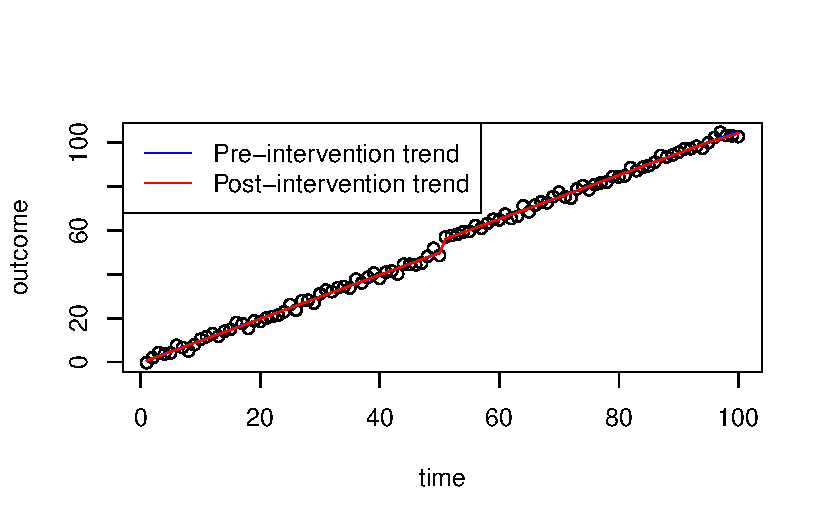
\includegraphics{ts_files/figure-pdf/unnamed-chunk-1-1.pdf}

}

\end{figure}

\hypertarget{prophet-package}{%
\section{Prophet Package}\label{prophet-package}}

\begin{itemize}
\tightlist
\item
  Developed by Facebook
\item
  Time series forecasting tool
\item
  Uses an additive regression model
\item
  Includes components for trend, seasonality, and holidays
\item
  Flexible and easy to use
\end{itemize}

\hypertarget{additive-regression-model}{%
\section{Additive Regression Model}\label{additive-regression-model}}

\begin{itemize}
\tightlist
\item
  Sum of individual effects
\item
  In Prophet, model is represented as: y(t) = g(t) + s(t) + h(t) + e(t)
\item
  g(t): trend component
\item
  s(t): seasonality component
\item
  h(t): holiday component
\item
  e(t): error term
\end{itemize}

\hypertarget{using-prophet-in-r}{%
\section{Using Prophet in R}\label{using-prophet-in-r}}

\hypertarget{step-1-install-and-load-the-prophet-package}{%
\subsection{Step 1: Install and load the Prophet
package}\label{step-1-install-and-load-the-prophet-package}}

\begin{itemize}
\tightlist
\item
  Prophet can be installed from CRAN
\item
  Open R console or RStudio
\item
  Install from CRAN using \texttt{install.packages("prophet")}
\item
  Load with \texttt{library(prophet)}
\end{itemize}

\begin{Shaded}
\begin{Highlighting}[]
\CommentTok{\# Install Prophet}
\FunctionTok{install.packages}\NormalTok{(}\StringTok{"prophet"}\NormalTok{)}

\CommentTok{\# Load Prophet}
\FunctionTok{library}\NormalTok{(prophet)}
\end{Highlighting}
\end{Shaded}

\hypertarget{step-2-prepare-the-data}{%
\subsection{Step 2: Prepare the data}\label{step-2-prepare-the-data}}

\begin{itemize}
\tightlist
\item
  Prophet requires data in specific format
\item
  Column for date/time named \texttt{ds}
\item
  Column for value to be forecasted named \texttt{y}
\item
  Split data into pre- and post-intervention periods
\end{itemize}

\begin{Shaded}
\begin{Highlighting}[]
\CommentTok{\# Load and prepare data}
\NormalTok{df }\OtherTok{\textless{}{-}} \FunctionTok{read\_csv}\NormalTok{(}\StringTok{"my\_data.csv"}\NormalTok{) }\SpecialCharTok{\%\textgreater{}\%}
  \FunctionTok{rename}\NormalTok{(}\AttributeTok{ds =}\NormalTok{ date, }\AttributeTok{y =}\NormalTok{ value)}

\CommentTok{\# Split data into pre{-} and post{-}intervention}
\NormalTok{intervention\_date }\OtherTok{\textless{}{-}} \FunctionTok{as.Date}\NormalTok{(}\StringTok{"2020{-}01{-}01"}\NormalTok{)}
\NormalTok{pre\_intervention }\OtherTok{\textless{}{-}}\NormalTok{ df }\SpecialCharTok{\%\textgreater{}\%} \FunctionTok{filter}\NormalTok{(ds }\SpecialCharTok{\textless{}}\NormalTok{ intervention\_date)}
\NormalTok{post\_intervention }\OtherTok{\textless{}{-}}\NormalTok{ df }\SpecialCharTok{\%\textgreater{}\%} \FunctionTok{filter}\NormalTok{(ds }\SpecialCharTok{\textgreater{}=}\NormalTok{ intervention\_date)}
\end{Highlighting}
\end{Shaded}

\hypertarget{step-3-create-a-prophet-model}{%
\subsection{Step 3: Create a Prophet
model}\label{step-3-create-a-prophet-model}}

\begin{itemize}
\tightlist
\item
  Use \texttt{prophet()} function to create model
\item
  Optional arguments to customize model
\item
  Specify seasonality, holidays, etc.
\item
  Fit model to pre-intervention data
\end{itemize}

\begin{Shaded}
\begin{Highlighting}[]
\CommentTok{\# Create Prophet model}
\NormalTok{m }\OtherTok{\textless{}{-}} \FunctionTok{prophet}\NormalTok{(pre\_intervention)}
\end{Highlighting}
\end{Shaded}

\hypertarget{step-4-make-predictions-and-estimate-impact}{%
\subsection{Step 4: Make predictions and estimate
impact}\label{step-4-make-predictions-and-estimate-impact}}

\begin{itemize}
\tightlist
\item
  Make predictions for post-intervention period
\item
  Calculate difference between predicted and observed values to estimate
  impact
\end{itemize}

\begin{Shaded}
\begin{Highlighting}[]
\CommentTok{\# Make predictions for post{-}intervention period}
\NormalTok{future }\OtherTok{\textless{}{-}} \FunctionTok{make\_future\_dataframe}\NormalTok{(m, }\AttributeTok{periods =} \FunctionTok{nrow}\NormalTok{(post\_intervention))}
\NormalTok{forecast }\OtherTok{\textless{}{-}} \FunctionTok{predict}\NormalTok{(m, future)}

\CommentTok{\# Calculate difference between predicted and observed values}
\NormalTok{impact }\OtherTok{\textless{}{-}}\NormalTok{ post\_intervention}\SpecialCharTok{$}\NormalTok{y }\SpecialCharTok{{-}}\NormalTok{ forecast}\SpecialCharTok{$}\NormalTok{yhat}
\end{Highlighting}
\end{Shaded}

\hypertarget{step-5-plot-results}{%
\subsection{Step 5: Plot results}\label{step-5-plot-results}}

\begin{itemize}
\tightlist
\item
  Plot pre- and post-intervention data and predictions
\end{itemize}

\begin{Shaded}
\begin{Highlighting}[]
\CommentTok{\# Plot results}
\FunctionTok{plot}\NormalTok{(m, forecast)}
\FunctionTok{points}\NormalTok{(post\_intervention}\SpecialCharTok{$}\NormalTok{ds, post\_intervention}\SpecialCharTok{$}\NormalTok{y)}
\end{Highlighting}
\end{Shaded}

\hypertarget{example-lung-cancer-asi-in-japan}{%
\section{Example: Lung Cancer ASI in
Japan}\label{example-lung-cancer-asi-in-japan}}

\hypertarget{the-data}{%
\subsection{The Data}\label{the-data}}

\begin{Shaded}
\begin{Highlighting}[]
\CommentTok{\# Set the seed for reproducibility}
\FunctionTok{set.seed}\NormalTok{(}\DecValTok{123}\NormalTok{)}

\CommentTok{\# Create a time series from 1980 to 2023}
\NormalTok{years }\OtherTok{\textless{}{-}} \FunctionTok{seq}\NormalTok{(}\DecValTok{1980}\NormalTok{, }\DecValTok{2023}\NormalTok{)}

\CommentTok{\# Generate a smooth trend in age{-}standardized incidence}
\NormalTok{lung\_cancer\_incidence }\OtherTok{\textless{}{-}} \DecValTok{100} \SpecialCharTok{+} \FunctionTok{seq}\NormalTok{(}\SpecialCharTok{{-}}\DecValTok{5}\NormalTok{, }\DecValTok{5}\NormalTok{, }\AttributeTok{length.out =} \FunctionTok{length}\NormalTok{(years))}

\CommentTok{\# Add some random noise to the data}
\NormalTok{lung\_cancer\_incidence }\OtherTok{\textless{}{-}}\NormalTok{ lung\_cancer\_incidence }\SpecialCharTok{+} \FunctionTok{rnorm}\NormalTok{(}\FunctionTok{length}\NormalTok{(years), }\AttributeTok{mean =} \DecValTok{0}\NormalTok{, }\AttributeTok{sd =} \DecValTok{1}\NormalTok{)}

\CommentTok{\# Simulate the banning of cigarettes in 2015}
\NormalTok{ban\_year }\OtherTok{\textless{}{-}} \DecValTok{2015}
\NormalTok{ban\_index }\OtherTok{\textless{}{-}} \FunctionTok{which}\NormalTok{(years }\SpecialCharTok{==}\NormalTok{ ban\_year)}

\CommentTok{\# Cause a slight decrease in lung cancer incidence after the ban}
\NormalTok{lung\_cancer\_incidence[ban\_index}\SpecialCharTok{:}\FunctionTok{length}\NormalTok{(lung\_cancer\_incidence)] }\OtherTok{\textless{}{-}}\NormalTok{ lung\_cancer\_incidence[ban\_index}\SpecialCharTok{:}\FunctionTok{length}\NormalTok{(lung\_cancer\_incidence)] }\SpecialCharTok{{-}} \FunctionTok{seq}\NormalTok{(}\DecValTok{0}\NormalTok{, }\DecValTok{5}\NormalTok{, }\AttributeTok{length.out =} \FunctionTok{length}\NormalTok{(lung\_cancer\_incidence[ban\_index}\SpecialCharTok{:}\FunctionTok{length}\NormalTok{(lung\_cancer\_incidence)]))}

\CommentTok{\# Create a data frame}
\NormalTok{data }\OtherTok{\textless{}{-}} \FunctionTok{data.frame}\NormalTok{(years, lung\_cancer\_incidence)}
\CommentTok{\# Load the ggplot2 library}
\FunctionTok{library}\NormalTok{(ggplot2)}

\CommentTok{\# Plot the data using ggplot}
\FunctionTok{ggplot}\NormalTok{(data, }\FunctionTok{aes}\NormalTok{(}\AttributeTok{x =}\NormalTok{ years, }\AttributeTok{y =}\NormalTok{ lung\_cancer\_incidence)) }\SpecialCharTok{+}
  \FunctionTok{geom\_line}\NormalTok{() }\SpecialCharTok{+}
  \FunctionTok{geom\_vline}\NormalTok{(}\AttributeTok{xintercept =} \DecValTok{2015}\NormalTok{, }\AttributeTok{linetype =} \StringTok{"dashed"}\NormalTok{) }\SpecialCharTok{+}
  \FunctionTok{labs}\NormalTok{(}\AttributeTok{title =} \StringTok{"Lung Cancer Incidence in Japan"}\NormalTok{,}
       \AttributeTok{subtitle =} \StringTok{"Simulated Impact of Cigarette Ban in 2015"}\NormalTok{,}
       \AttributeTok{x =} \StringTok{"Year"}\NormalTok{,}
       \AttributeTok{y =} \StringTok{"Lung Cancer Incidence"}\NormalTok{)}
\end{Highlighting}
\end{Shaded}

\begin{figure}[H]

{\centering 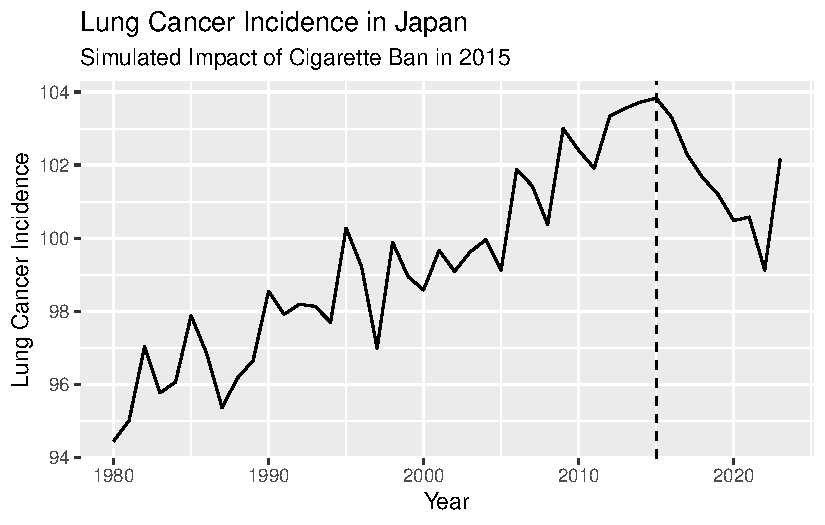
\includegraphics{ts_files/figure-pdf/unnamed-chunk-2-1.pdf}

}

\end{figure}

\hypertarget{step-1-load-prophet}{%
\subsection{Step 1: Load Prophet}\label{step-1-load-prophet}}

\begin{Shaded}
\begin{Highlighting}[]
\FunctionTok{library}\NormalTok{(prophet)}
\end{Highlighting}
\end{Shaded}

\begin{verbatim}
Warning: package 'prophet' was built under R version 4.2.3
\end{verbatim}

\begin{verbatim}
Loading required package: Rcpp
\end{verbatim}

\begin{verbatim}
Loading required package: rlang
\end{verbatim}

\begin{Shaded}
\begin{Highlighting}[]
\FunctionTok{library}\NormalTok{(prophet)}
\end{Highlighting}
\end{Shaded}

\hypertarget{step-2-prepare-the-data-1}{%
\subsection{Step 2: Prepare the Data}\label{step-2-prepare-the-data-1}}

\begin{Shaded}
\begin{Highlighting}[]
\NormalTok{data}
\end{Highlighting}
\end{Shaded}

\begin{verbatim}
   years lung_cancer_incidence
1   1980              94.43952
2   1981              95.00238
3   1982              97.02382
4   1983              95.76818
5   1984              96.05952
6   1985              97.87786
7   1986              96.85627
8   1987              95.36285
9   1988              96.17361
10  1989              96.64736
11  1990              98.54966
12  1991              97.91795
13  1992              98.19147
14  1993              98.13394
15  1994              97.69997
16  1995             100.27529
17  1996              99.21878
18  1997              96.98687
19  1998              99.88740
20  1999              98.94581
21  2000              98.58334
22  2001              99.66575
23  2002              99.09027
24  2003              99.61995
25  2004              99.95636
26  2005              99.12726
27  2006             101.88430
28  2007             101.43244
29  2008             100.37349
30  2009             102.99800
31  2010             102.40321
32  2011             101.91423
33  2012             103.33699
34  2013             103.55255
35  2014             103.72856
36  2015             103.82818
37  2016             103.30101
38  2017             102.29274
39  2018             101.65625
40  2019             101.18930
41  2020             100.48262
42  2021             100.57697
43  2022              99.12705
44  2023             102.16896
\end{verbatim}

\hypertarget{step-2-prepare-the-data-2}{%
\subsection{Step 2: Prepare the data}\label{step-2-prepare-the-data-2}}

\begin{itemize}
\tightlist
\item
  Prepare the data names
\item
  Split it to pre- and post-intervention periods
\end{itemize}

\begin{Shaded}
\begin{Highlighting}[]
\NormalTok{data}\SpecialCharTok{$}\NormalTok{ds }\OtherTok{\textless{}{-}} \FunctionTok{as.Date}\NormalTok{(}\FunctionTok{paste0}\NormalTok{(data}\SpecialCharTok{$}\NormalTok{years, }\StringTok{"{-}01{-}01"}\NormalTok{))}
\NormalTok{data}\SpecialCharTok{$}\NormalTok{y }\OtherTok{\textless{}{-}}\NormalTok{ data}\SpecialCharTok{$}\NormalTok{lung\_cancer\_incidence}

\CommentTok{\# Spliting}
\NormalTok{before }\OtherTok{\textless{}{-}}\NormalTok{ data[data}\SpecialCharTok{$}\NormalTok{years }\SpecialCharTok{\textless{}=} \DecValTok{2015}\NormalTok{,]}
\NormalTok{after }\OtherTok{\textless{}{-}}\NormalTok{ data[data}\SpecialCharTok{$}\NormalTok{years }\SpecialCharTok{\textgreater{}} \DecValTok{2015}\NormalTok{,]}
\end{Highlighting}
\end{Shaded}

\begin{Shaded}
\begin{Highlighting}[]
\NormalTok{data}\SpecialCharTok{$}\NormalTok{ds }\OtherTok{\textless{}{-}} \FunctionTok{as.Date}\NormalTok{(}\FunctionTok{paste0}\NormalTok{(data}\SpecialCharTok{$}\NormalTok{years, }\StringTok{"{-}01{-}01"}\NormalTok{))}
\NormalTok{data}\SpecialCharTok{$}\NormalTok{y }\OtherTok{\textless{}{-}}\NormalTok{ data}\SpecialCharTok{$}\NormalTok{lung\_cancer\_incidence}
\NormalTok{before }\OtherTok{\textless{}{-}}\NormalTok{ data[data}\SpecialCharTok{$}\NormalTok{years }\SpecialCharTok{\textless{}=} \DecValTok{2015}\NormalTok{,]}
\NormalTok{after }\OtherTok{\textless{}{-}}\NormalTok{ data[data}\SpecialCharTok{$}\NormalTok{years }\SpecialCharTok{\textgreater{}} \DecValTok{2015}\NormalTok{,]}
\end{Highlighting}
\end{Shaded}

\hypertarget{step-3-create-a-prophet-model-1}{%
\subsection{Step 3: Create a Prophet
model}\label{step-3-create-a-prophet-model-1}}

\begin{Shaded}
\begin{Highlighting}[]
\NormalTok{m }\OtherTok{\textless{}{-}} \FunctionTok{prophet}\NormalTok{(before)}
\end{Highlighting}
\end{Shaded}

\begin{Shaded}
\begin{Highlighting}[]
\NormalTok{m }\OtherTok{\textless{}{-}} \FunctionTok{prophet}\NormalTok{(before)}
\end{Highlighting}
\end{Shaded}

\begin{verbatim}
Disabling weekly seasonality. Run prophet with weekly.seasonality=TRUE to override this.
\end{verbatim}

\begin{verbatim}
Disabling daily seasonality. Run prophet with daily.seasonality=TRUE to override this.
\end{verbatim}

\hypertarget{step-4-forecasting}{%
\subsection{Step 4: Forecasting}\label{step-4-forecasting}}

\begin{Shaded}
\begin{Highlighting}[]
\NormalTok{future }\OtherTok{\textless{}{-}} \FunctionTok{make\_future\_dataframe}\NormalTok{(m, }\AttributeTok{periods =} \FunctionTok{length}\NormalTok{(test\_data}\SpecialCharTok{$}\NormalTok{years), }\AttributeTok{freq =} \StringTok{"year"}\NormalTok{)}
\NormalTok{forecast }\OtherTok{\textless{}{-}} \FunctionTok{predict}\NormalTok{(m, future)}
\NormalTok{forecast}\SpecialCharTok{$}\NormalTok{ds }\OtherTok{\textless{}{-}} \FunctionTok{as.Date}\NormalTok{(forecast}\SpecialCharTok{$}\NormalTok{ds)}
\end{Highlighting}
\end{Shaded}

\begin{Shaded}
\begin{Highlighting}[]
\NormalTok{future }\OtherTok{\textless{}{-}} \FunctionTok{make\_future\_dataframe}\NormalTok{(m, }\AttributeTok{periods =} \FunctionTok{length}\NormalTok{(after}\SpecialCharTok{$}\NormalTok{years), }\AttributeTok{freq =} \StringTok{"year"}\NormalTok{)}
\NormalTok{forecast }\OtherTok{\textless{}{-}} \FunctionTok{predict}\NormalTok{(m, future)}
\NormalTok{forecast}\SpecialCharTok{$}\NormalTok{ds }\OtherTok{\textless{}{-}} \FunctionTok{as.Date}\NormalTok{(forecast}\SpecialCharTok{$}\NormalTok{ds)}
\end{Highlighting}
\end{Shaded}

\hypertarget{step-5-plot-results-1}{%
\subsection{Step 5: Plot results}\label{step-5-plot-results-1}}

\begin{Shaded}
\begin{Highlighting}[]
\FunctionTok{ggplot}\NormalTok{() }\SpecialCharTok{+}
  \FunctionTok{geom\_line}\NormalTok{(}\AttributeTok{data =}\NormalTok{ data, }\FunctionTok{aes}\NormalTok{(}\AttributeTok{x =}\NormalTok{ ds, }\AttributeTok{y =}\NormalTok{ y), }\AttributeTok{color =} \StringTok{"blue"}\NormalTok{) }\SpecialCharTok{+}
  \FunctionTok{geom\_line}\NormalTok{(}\AttributeTok{data =}\NormalTok{ forecast, }\FunctionTok{aes}\NormalTok{(}\AttributeTok{x =}\NormalTok{ ds, }\AttributeTok{y =}\NormalTok{ yhat), }\AttributeTok{color =} \StringTok{"red"}\NormalTok{, }\AttributeTok{linetype =} \StringTok{"dashed"}\NormalTok{) }\SpecialCharTok{+}  \FunctionTok{geom\_vline}\NormalTok{(}\AttributeTok{xintercept =} \DecValTok{2015}\NormalTok{, }\AttributeTok{linetype =} \StringTok{"dashed"}\NormalTok{) }\SpecialCharTok{+}
  \FunctionTok{labs}\NormalTok{(}\AttributeTok{title =} \StringTok{"Lung Cancer Incidence in Japan"}\NormalTok{,}
       \AttributeTok{subtitle =} \StringTok{"Observed vs. Counterfactual Without Cigarette Ban"}\NormalTok{,}
       \AttributeTok{x =} \StringTok{"Year"}\NormalTok{,}
       \AttributeTok{y =} \StringTok{"Lung Cancer Incidence"}\NormalTok{)}
\end{Highlighting}
\end{Shaded}

\begin{Shaded}
\begin{Highlighting}[]
\FunctionTok{ggplot}\NormalTok{() }\SpecialCharTok{+}
  \FunctionTok{geom\_line}\NormalTok{(}\AttributeTok{data =}\NormalTok{ data, }\FunctionTok{aes}\NormalTok{(}\AttributeTok{x =}\NormalTok{ ds, }\AttributeTok{y =}\NormalTok{ y), }\AttributeTok{color =} \StringTok{"blue"}\NormalTok{) }\SpecialCharTok{+}
  \FunctionTok{geom\_line}\NormalTok{(}\AttributeTok{data =}\NormalTok{ forecast, }\FunctionTok{aes}\NormalTok{(}\AttributeTok{x =}\NormalTok{ ds, }\AttributeTok{y =}\NormalTok{ yhat), }\AttributeTok{color =} \StringTok{"red"}\NormalTok{, }\AttributeTok{linetype =} \StringTok{"dashed"}\NormalTok{) }\SpecialCharTok{+}  \FunctionTok{geom\_vline}\NormalTok{(}\AttributeTok{xintercept =} \DecValTok{2015}\NormalTok{, }\AttributeTok{linetype =} \StringTok{"dashed"}\NormalTok{) }\SpecialCharTok{+}
  \FunctionTok{labs}\NormalTok{(}\AttributeTok{title =} \StringTok{"Lung Cancer Incidence in Japan"}\NormalTok{,}
       \AttributeTok{subtitle =} \StringTok{"Observed vs. Counterfactual Without Cigarette Ban"}\NormalTok{,}
       \AttributeTok{x =} \StringTok{"Year"}\NormalTok{,}
       \AttributeTok{y =} \StringTok{"Lung Cancer Incidence"}\NormalTok{)}
\end{Highlighting}
\end{Shaded}

\begin{figure}[H]

{\centering 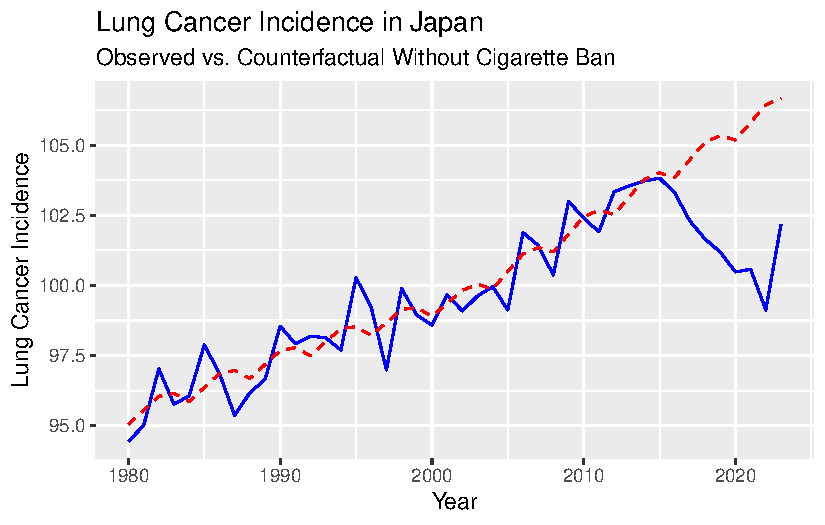
\includegraphics{ts_files/figure-pdf/unnamed-chunk-8-1.pdf}

}

\end{figure}



\end{document}
